%------------------------------------------%
%
% Cannabis Data Science #63
%
% Date: 4/27/2022
%
%------------------------------------------%
\documentclass[xcolor={dvipsnames}]{beamer}
\hypersetup{pdfpagemode = FullScreen}
\mode<presentation>{
  \usetheme{Boadilla}
  \usecolortheme{orchid}
  \usefonttheme{default}
  \setbeamertemplate{navigation symbols}{}
  \setbeamertemplate{caption}[numbered]
}
\setbeamersize{
  text margin left = 0.5in,
  text margin right = 0.5in
}

%------------------------------------------%
% Title
%------------------------------------------%
\title[\textbf{Cannabis Data Science \#63}]{}
\author{Cannlytics}
\institute[]{\Large Cannabis Data Science \#63}
\date{April \nth{27}, 2022}

%------------------------------------------%
% Packages
%------------------------------------------%
\usepackage[english]{babel}
\usepackage[utf8x]{inputenc}
\usepackage{tikz} % For styling.
\usepackage{xparse}

%------------------------------------------%
% Colors
%------------------------------------------%
\definecolor{Green}{RGB}{34, 153, 84}
\definecolor{LightGreen}{RGB}{218, 247, 166}
\definecolor{DarkGreen}{RGB}{2, 48, 32}
\definecolor{Orange}{RGB}{255, 87, 51}
\definecolor{DarkOrange}{RGB}{199, 0, 57}
\definecolor{Yellow}{RGB}{255, 195, 0}

%------------------------------------------%
% Theme
%------------------------------------------%
\setbeamercolor*{palette primary}{bg=LightGreen, fg=DarkGreen}
\setbeamercolor*{palette secondary}{bg=LightGreen, fg=DarkGreen}
\setbeamercolor*{palette tertiary}{bg=LightGreen, fg=DarkGreen}

%------------------------------------------%
% Packages
%------------------------------------------%
\usepackage{amsmath}
\renewcommand*\footnoterule{} % No separating line on footnote.
\usepackage{mathtools} % For annotating equations.
\usepackage{hhline} % for double bars.
\usepackage[super]{nth} % For formatting 1st, 2nd, 3rd, etc.
\usepackage{graphicx, caption, subcaption}
\usepackage{setspace}

%------------------------------------------%
% Commands
%------------------------------------------%

% Top space.
\newcommand\T{\rule{0pt}{2.5ex}}

% Bottom space.
\newcommand\B{\rule[-1.25ex]{0pt}{0pt}}

% Blocks.
\newenvironment<>{Block}[2][.9\textwidth]
  {\setlength{\textwidth}{#1}
  \begin{actionenv}#3
    \def\insertblocktitle{#2}\par
    \usebeamertemplate{block begin}}
  {\par\usebeamertemplate{block end}
  \end{actionenv}}

% Balls.
\defbeamertemplate{enumerate item}{largeball}
{\begin{pgfpicture}{-1ex}{-0.65ex}{1.5ex}{1.5ex}
\usebeamercolor[fg]{item projected}
{\pgftransformscale{2.5}\pgftext{\Large\pgfuseshading{bigsphere}}}
{\pgftransformshift{\pgfpoint{0pt}{0.5pt}}
\pgftext{\usebeamerfont*{item projected}\small\insertenumlabel}}
\end{pgfpicture}}

% Fancy arrows.
\NewDocumentCommand\UpArrow{O{2.0ex} O{black}}{%
   \mathrel{\tikz[baseline] \draw [->, line width=0.5pt, #2] (0,0) -- ++(0,#1);}} % Fancy up-arrow.
\NewDocumentCommand\DownArrow{O{2.0ex} O{black}}{%
   \mathrel{\tikz[baseline] \draw [<-, line width=0.5pt, #2] (0,0) -- ++(0,#1);}} % Fancy down-arrow.

% Equations with numbers on the left.
\makeatletter
\newcommand{\LeftEqNo}{\let\veqno\@@leqno}
\makeatother


\defbeamertemplate*{title page}{customized}[1][]
{
  \usebeamerfont{title}\inserttitle\par
  \bigskip
  \vspace{0.5\baselineskip}
  \usebeamerfont{institute}\insertinstitute\par
  \vspace{0.5\baselineskip}
  {\small\usebeamerfont{date}\insertdate\par}
  \usebeamercolor[fg]{titlegraphic}\inserttitlegraphic
}

%------------------------------------------%
%
% Presentation
%
%------------------------------------------%
\begin{document}

% Title page.
\begin{frame}{}

% Background
\tikz[remember picture, overlay]
\node[opacity=1.0, inner sep=0pt] at (current page.center){
  
\includegraphics[height=\paperheight, width=\paperwidth]{images/presentation-cover.pdf}
};

% Title
\vspace*{4\baselineskip}

\includegraphics[scale=0.375]{images/logo.pdf}
\vspace*{-2\baselineskip}
\titlepage
\end{frame}

%------------------------------------------%
% Introduction
%------------------------------------------%

\begin{frame}{}

\begin{figure}
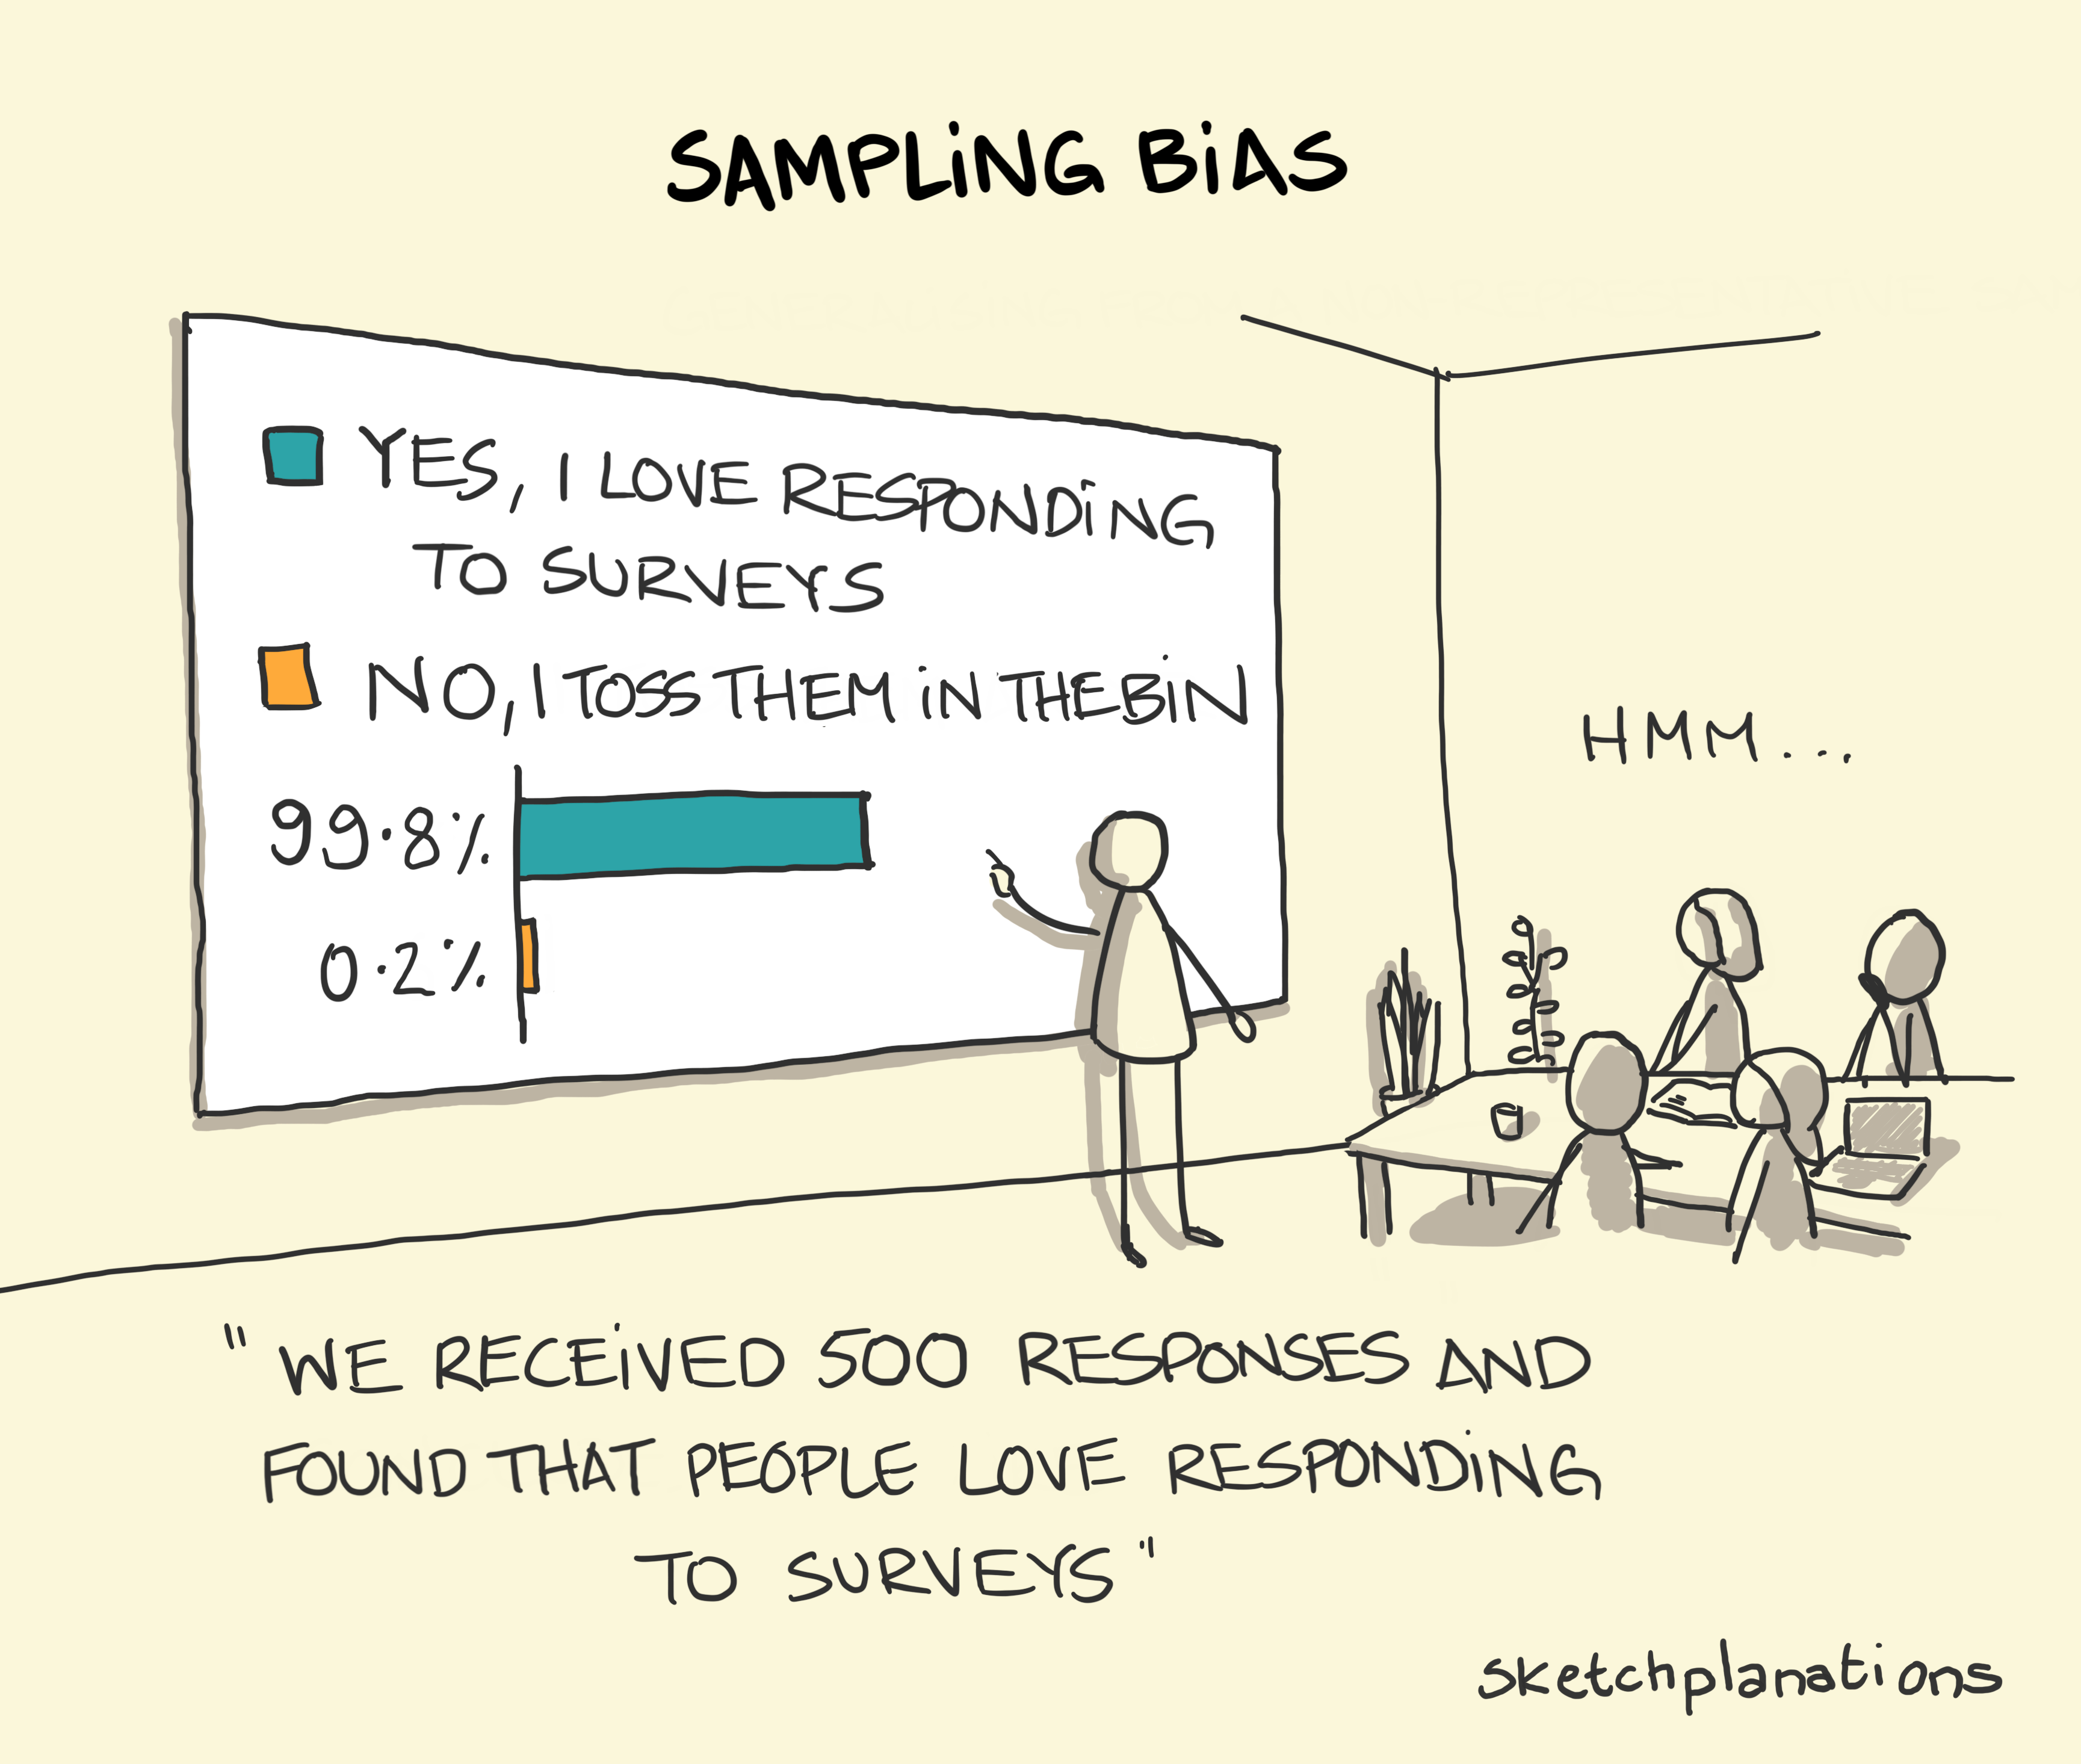
\includegraphics[width=0.8\textwidth]{images/sketchplanations-sampling-bias.png}
\end{figure}

{\tiny Author: Sketchplanations https://sketchplanations.com/\\
License: CC BY-NC 4.0 http://creativecommons.org/licenses/by-nc/4.0/ }

\end{frame}

%------------------------------------------%
% Consumer Demand
%------------------------------------------%

\begin{frame}{Consumer Demand}

\begin{minipage}{0.5\textwidth}

% Supply and Demand
\begin{figure}
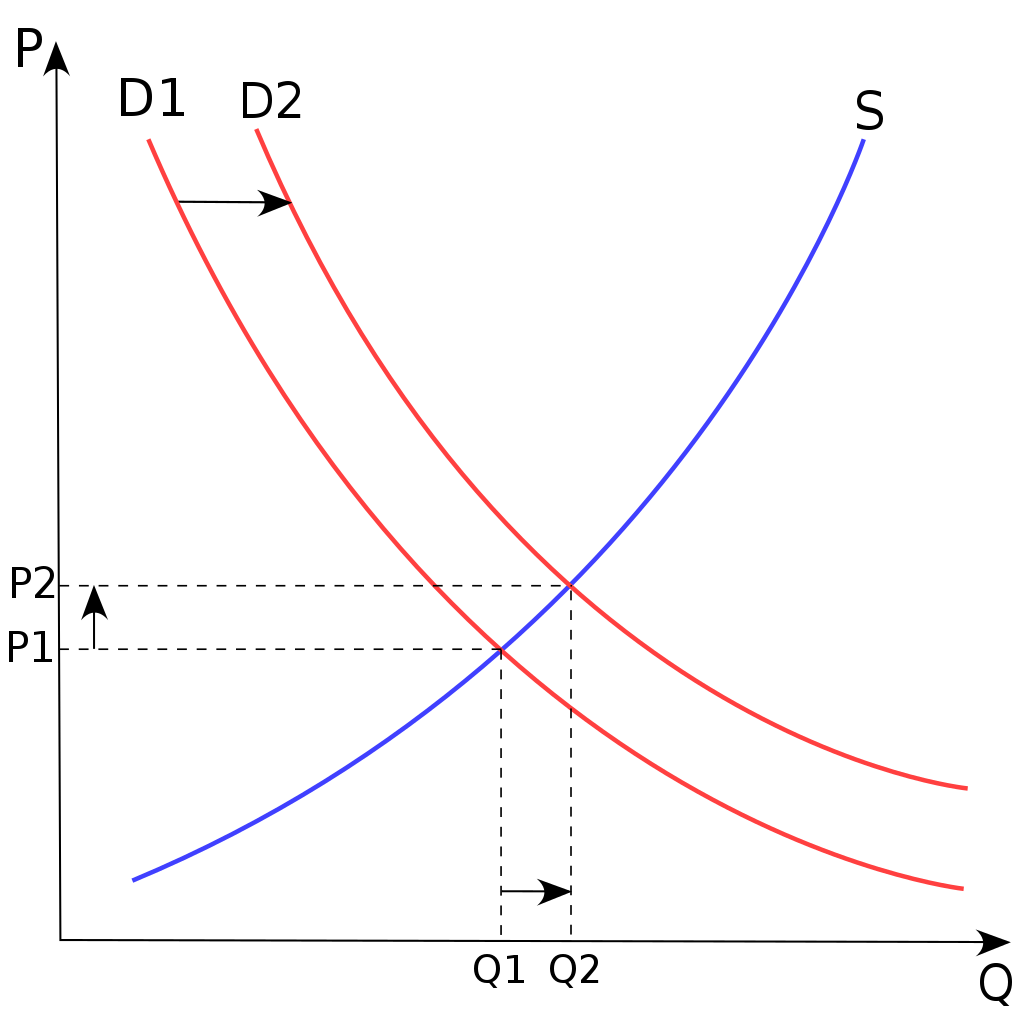
\includegraphics[width=2in]{images/supply-and-demand.png}
\end{figure}

{\footnotesize A shift in demand, with equilibrium price, $P$, and quantity, $Q$, increasing.}

\vspace{.5\baselineskip}

{\tiny Author: Paweł Zdziarski (faxe), Astarot\\
License: CC BY-SA 3.0 \\http://creativecommons.org/licenses/by-sa/3.0/}

\end{minipage}%
\begin{minipage}{0.5\textwidth}

\vspace{-12\baselineskip}

% Question of the day
\begin{center}
\begin{minipage}{\linewidth}
\begin{Block}{Question of the day.}

\vspace{.5\baselineskip}
\begin{itemize}

\item What is {\bfseries consumer demand} for {\color{Green} \underline{cannabis}} \\in the US?

\end{itemize}

\vspace{.5\baselineskip}

\end{Block}
\end{minipage}
\end{center}


\end{minipage}

\end{frame}

%------------------------------------------%
% Question and Hypothesis
%------------------------------------------%
%\section{Question and Hypothesis}
%\begin{frame}{Question and Hypothesis}
%
%% Question of the day
%\begin{center}
%\begin{minipage}{.9\linewidth}
%\begin{Block}{Question of the day.}
%
%\vspace{.5\baselineskip}
%\begin{itemize}
%
%\item What is {\bfseries consumer demand} in the US?
%
%\end{itemize}
%
%\vspace{.5\baselineskip}
%
%\end{Block}
%\end{minipage}
%\end{center}
%
%\end{frame}

%------------------------------------------%

%An application programming interface (API) is a connection between computers or between computer programs.



% 
% Christopher J. Date
% Helped design SQL/DS, which implemented the SQL database-query language.
% Coined the term API in `The Relational and Network Approaches: Comparison of the Application Programming Interface` (1974).

% Google LLC v. Oracle America, Inc.

%------------------------------------------%
% Census
%------------------------------------------%

\begin{frame}{Let's check the Census!}


\begin{figure}
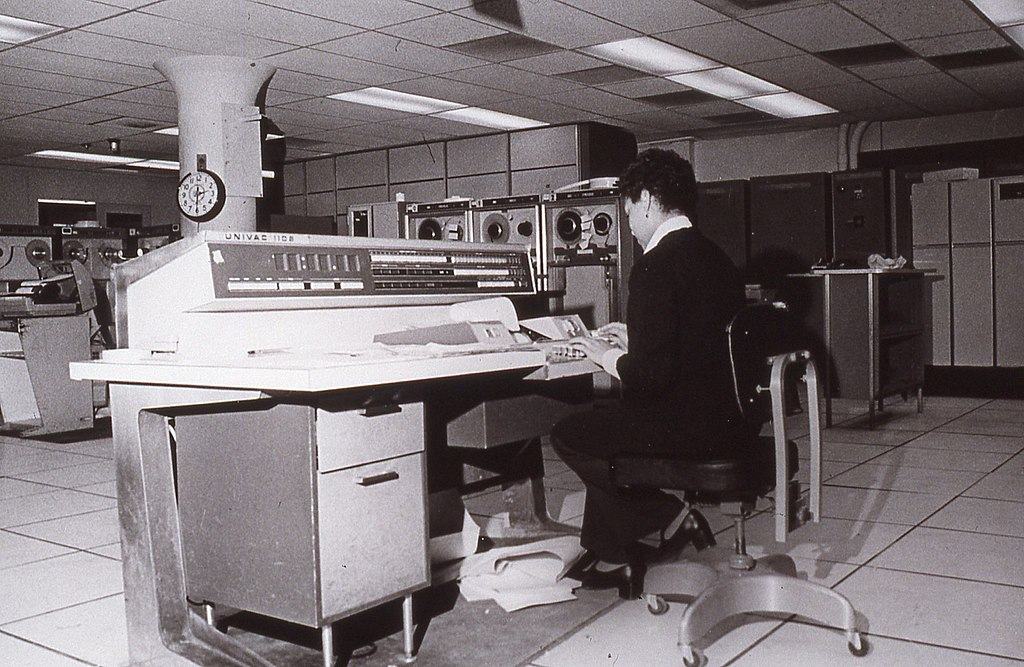
\includegraphics[width=0.9\textwidth]{images/census-bureau-employee.jpg}
\end{figure}

A Census Bureau employee (1970s) operating a UNIVAC 1100 series computer, likely processing data from the 1970 Census.

\end{frame}


%------------------------------------------%
% APIs + Cron jobs = AI
%------------------------------------------%

% By mapping the features and capabilities of one language to an interface implemented in another language, a language binding allows a library or service written in one language to be used when developing in another language.

%------------------------------------------%
% Takeaway
%------------------------------------------%
\section{Takeaway}
\begin{frame}{}

\vspace{0.5\baselineskip}

\begin{center}
\begin{minipage}{3.85in}

% Thank you.

\includegraphics[width=.25in]{images/prayer.png} {\Large \textbf{Thank you for coming.}}\\[-0.75\baselineskip]

\begin{center}
\begin{minipage}{\linewidth}
\begin{Block}{Insight of the Day}

\vspace{0.5\baselineskip}

\begin{itemize}

\item Stand on the shoulders of giants.

\vspace{0.5\baselineskip}

\end{itemize}

\end{Block}
\end{minipage}
\end{center}

\vfill

\end{minipage}
\end{center}

\vspace{0.5\baselineskip}

{\large What is on your mind for next week?}\\

\end{frame}


%------------------------------------------%
% Fin.
%------------------------------------------%
\end{document}
